\section{Experimentación}

Quisimos estudiar el comportamiento de nuestros algoritmos con instancias reales. Para ello corrimos el programa con instancias generadas aleatoriamente, siguiendo una distribución uniforme. Generamos casos de test con distintos valores de N (cantidad de elementos) para cada algoritmo. Como nuestras instancias fueron generadas aleatoriamente, corrimos numerosas veces los algoritmos y tomamos el promedio de sus tiempos, evitando así caer en casos extremos.
Una vez que obtuvimos los datos, comparamos nuestros resultados con las cotas asintóticas calculadas previamente .


\subsection{Experimentación sobre el algoritmo de Fuerza Bruta}
Para el algoritmo de Fuerza Bruta, comenzamos con un análisis del caso en el que no aplicamos ninguna poda. Como vimos en la sección anterior, tenemos una cota teórica de O($n*2^{n}$). Para ver que tan bien se ajusta nuestro algoritmo a ésta cota, generamos nuestros casos de test variando N entre 0 y 30. Veamos los resultados:

\begin{figure}[!htb]
   \begin{minipage}{0.6\textwidth}
     \centering
     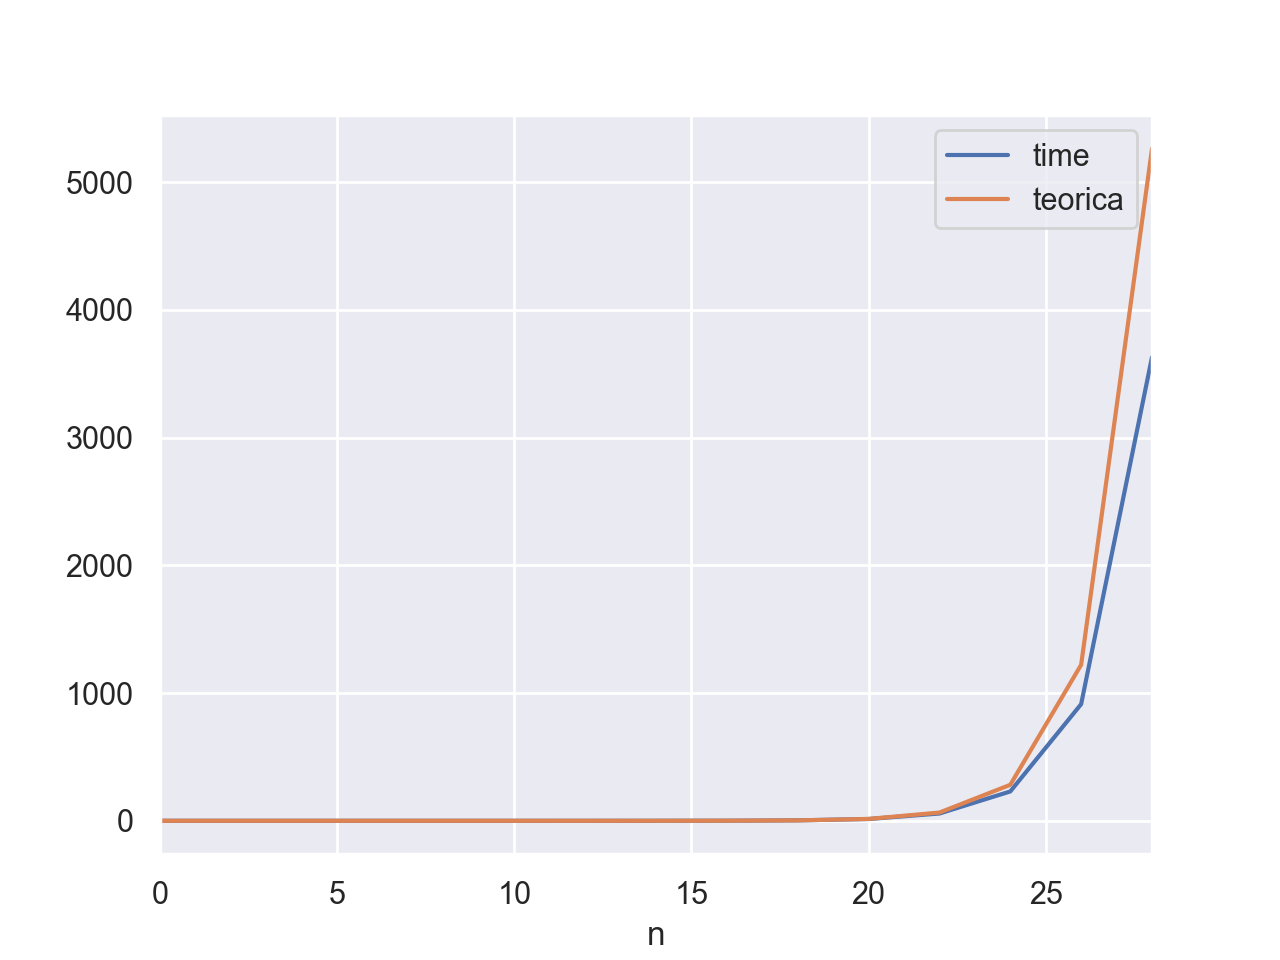
\includegraphics[width=1\linewidth]{img/sinPodas1}
     \caption{Comparación del gráfico de los resultados contra la cota teórica}
   \end{minipage}\hfill
   \begin{minipage}{0.6\textwidth}
     \centering
     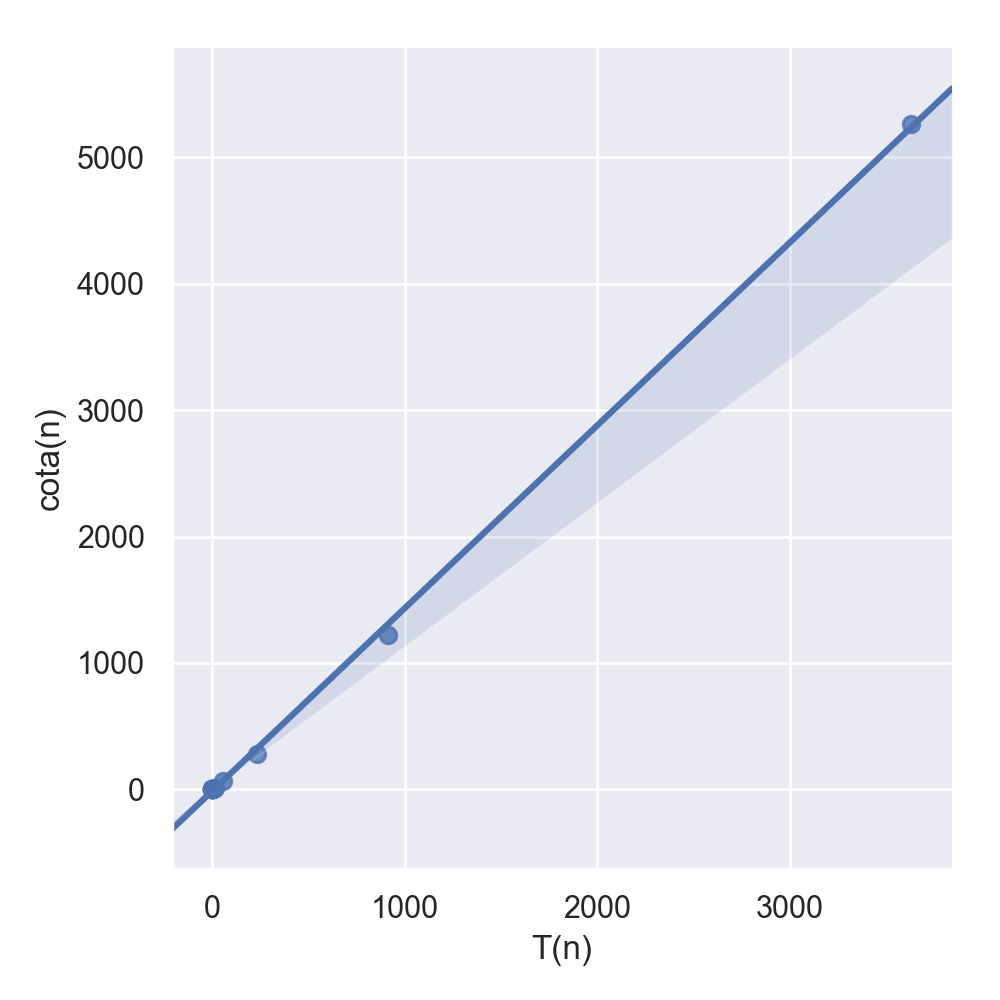
\includegraphics[width=1\linewidth]{img/sinPodas2}
     \caption{Correlación entre algoritmo y cota teórica}
   \end{minipage}
\end{figure}

Como podemos observar en el primer gráfico, podemos observar que la cota teórica tiene un crecimiento un poco más acelerado que nuestros datos. Esto es un resultado que nos sorprende, ya que como vimos antes, la complejidad de éste algoritmo se puede calcular de manera sencilla. Creemos que esta diferencia puede deberse a que no fue posible experimentar demasiados valores de N, dado que el tiempo de ejecución no nos lo permitió.
\newline
Ésta misma diferencia se ve plasmada en el segundo gráfico. En este caso, podemos ver que nuestros datos tienen una correlación positiva con la cota que, aunque es bastante fuerte, no es tan ajustada como por ejemplo en el algoritmo de Meet in the Middle.

\subsection{Experimentación sobre el algoritmo de Meet in the Middle}

En el caso de Meet in the Middle, variamos N en un rango de 0 a 50, y comparamos nuestros resultados con la cota teórica O($n*2^{n/2}$). Los siguientes gráficos muestran nuestros resultados:

\begin{figure}[!htb]
   \begin{minipage}{0.6\textwidth}
     \centering
     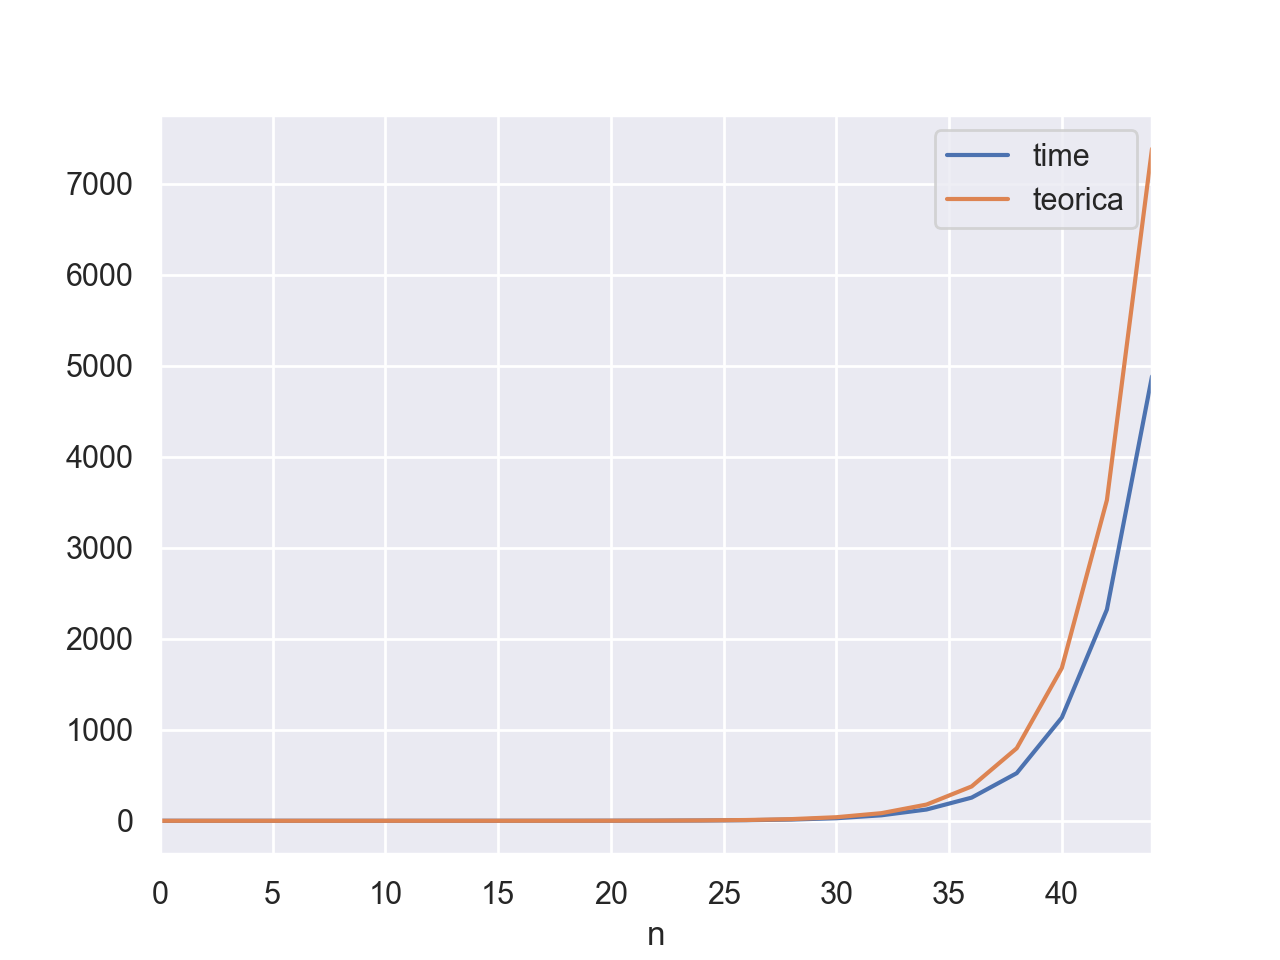
\includegraphics[width=1\linewidth]{img/Middle1}
     \caption{Comparación del gráfico de los resultados contra la cota teórica}
   \end{minipage}\hfill
   \begin{minipage}{0.6\textwidth}
     \centering
     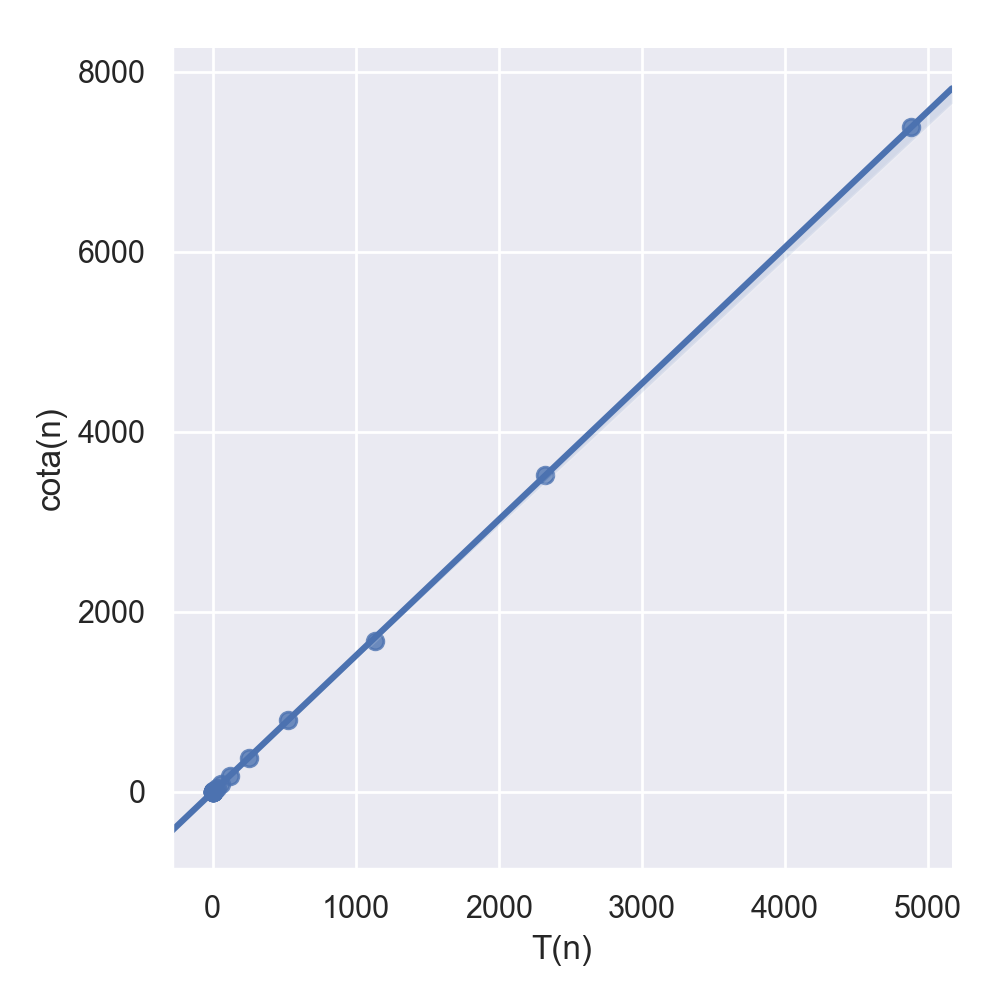
\includegraphics[width=1\linewidth]{img/Middle2}
     \caption{Correlación entre algoritmo y cota teórica}
   \end{minipage}
\end{figure}

Como podemos observar en el primer gráfico, parecería ser que el tiempo de ejecución se ajusta fuertemente a la cota teórica. Ambas funciones parecen tener un crecimiento similar, pero podemos corroborar esto más apropiadamente con el segundo gráfico. Aquí, vemos que nuestros datos tienen una correlación positiva casi perfecta con la cota teórica. La recta de cuadrados mínimos cubre casi perfectamente a nuestros datos.
\label{sec:experimentacion}



\subsection{Experimentación sobre el algoritmo de Backtracking}
Para el algoritmo de backtracking, comenzamos con un análisis del caso en el que no aplicamos ninguna poda. Como vimos en la sección anterior, tenemos una cota teórica de O($n*2^{n}$). Para ver que tan bien se ajusta nuestro algoritmo a ésta cota, generamos nuestros casos de test variando N entre 0 y 30. Veamos los resultados:

\begin{figure}[!htb]
   \begin{minipage}{0.6\textwidth}
     \centering
     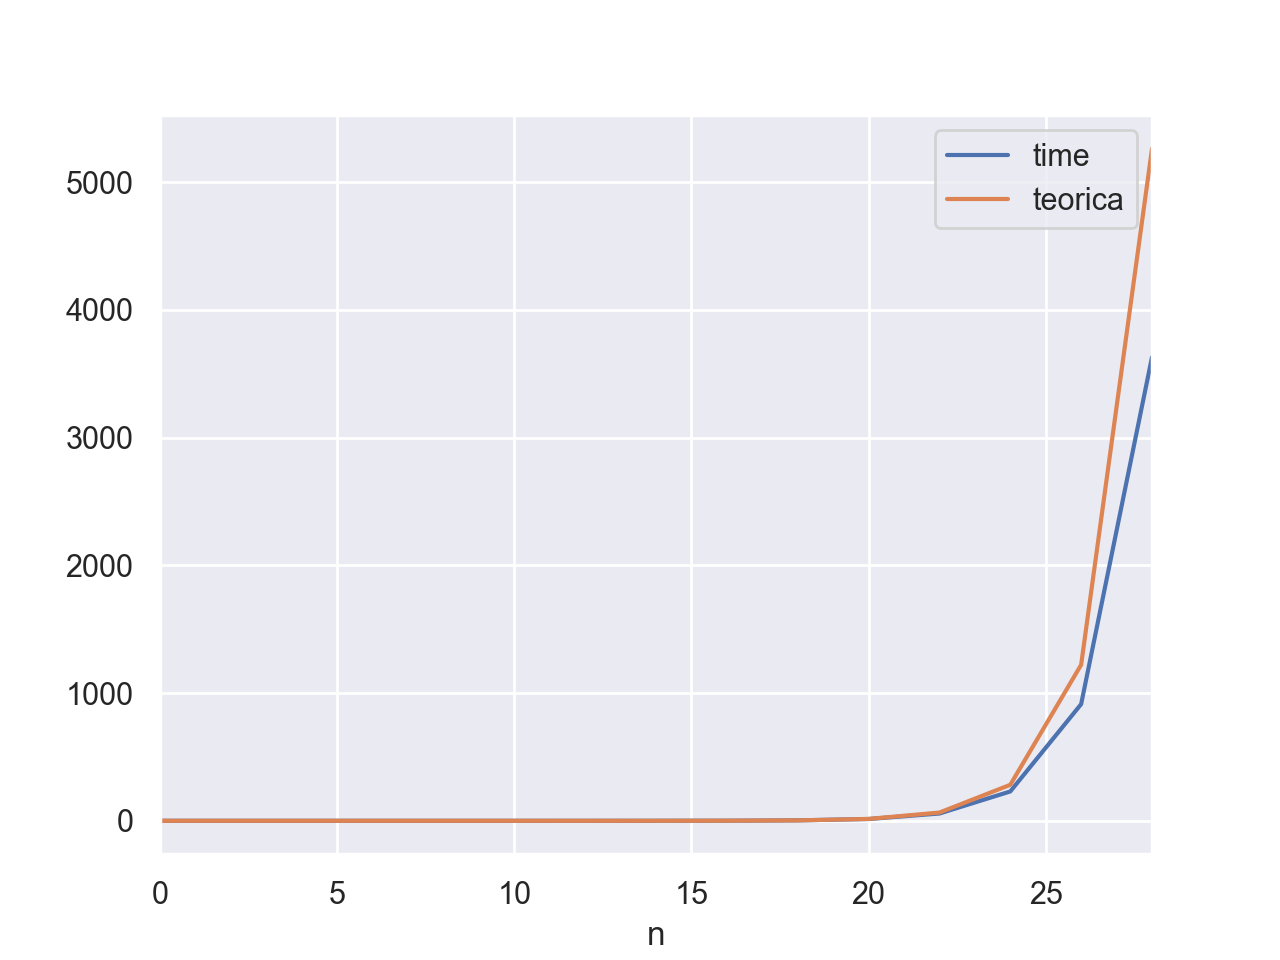
\includegraphics[width=1\linewidth]{img/sinPodas1}
     \caption{Comparación del gráfico de los resultados contra la cota teórica}
   \end{minipage}\hfill
   \begin{minipage}{0.6\textwidth}
     \centering
     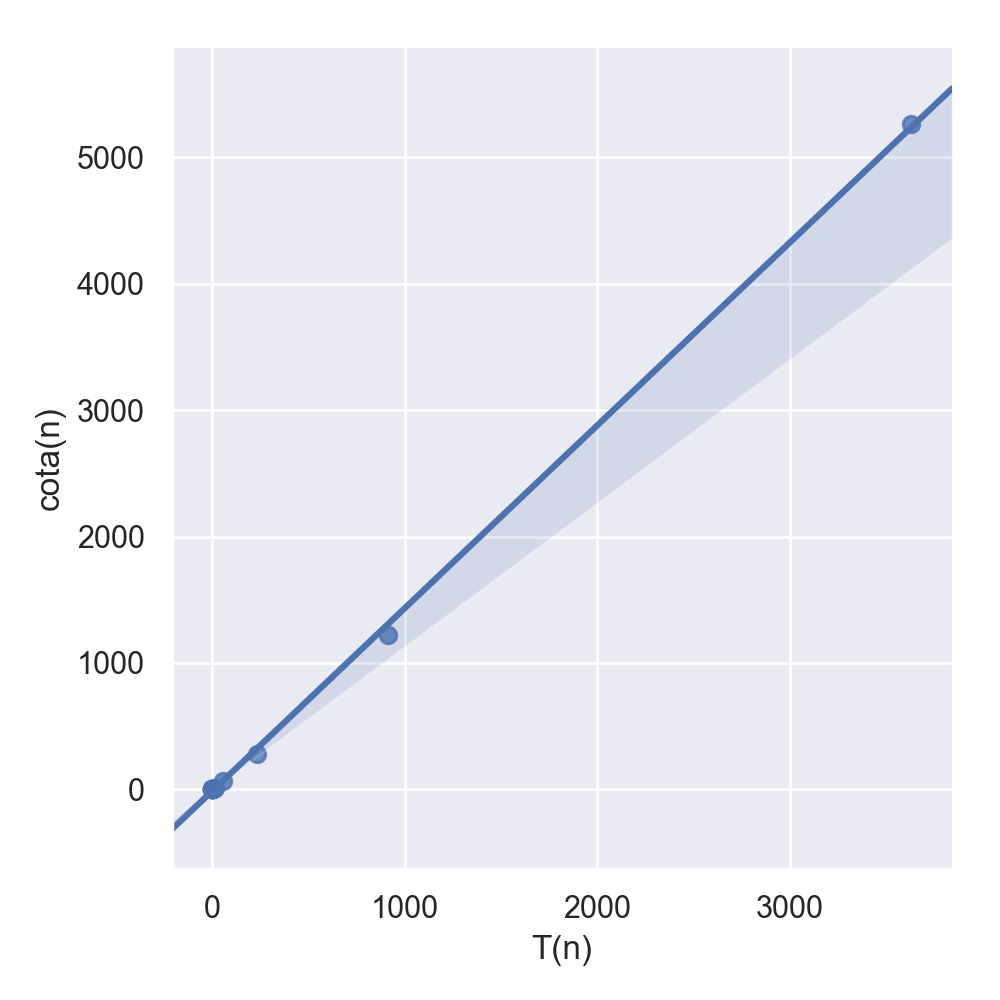
\includegraphics[width=1\linewidth]{img/sinPodas2}
     \caption{Correlación entre algoritmo y cota teórica}
   \end{minipage}
\end{figure}

Como podemos observar en el primer gráfico, podemos observar que la cota teórica tiene un crecimiento un poco más acelerado que nuestros datos. Esto es un resultado que nos sorprende, ya que como vimos antes, la complejidad de éste algoritmo se puede calcular de manera sencilla. Creemos que esta diferencia puede deberse a que no fue posible experimentar demasiados valores de N, dado que el tiempo de ejecución no nos lo permitió.
\newline
Ésta misma diferencia se ve plasmada en el segundo gráfico. En este caso, podemos ver que nuestros datos tienen una correlación positiva con la cota que, aunque es bastante fuerte, no es tan ajustada como por ejemplo en el algoritmo de Meet in the Middle.
